\section{Experimental Evaluation}\label{sec:exp}
We evaluate our techniques on two real-world trajectory datasets: \pt{}, \sz{} and \cd{}.
\pt{}~\cite{pt} contains a total of 2.39 million taxi trajectories and 75.67 million of GPS points, and the longest trajectory has 3,490 GPS points.
\sz{}~\cite{sz} consists of 3.07 million taxi trajectories with 53.53 million GPS points, and the longest trajectory has 2,268 GPS points. 
\cd{}~\cite{cd} consists of \QM{0.28} million taxi trajectories with \QM{6.69} million GPS points, and the longest trajectory has \QM{4025} GPS points.  All experiments are conducted on a machine with an Intel i7-8700 CPU, 24 GB memory and an NVIDIA GeForce GTX1080 GPU with 8 GB on-chip memory, running on Windows 10. All methods are implemented in Java 1.8, and the Processing 3 library~\cite{p3} is used for rendering. All datasets and source codes required to reproduce our results are available at~\cite{code}.

%\REPORT{
This section is organized as follows.
In Section~\ref{sec:case}, we present several case studies of the visualization results on the \pt{} datasets to demonstrate the merits of our methods.
% In Section~\ref{sec:case}, we evaluate the effectiveness of our proposal by the case studies on \pt{} and \sz{} trajectory dataset, respectively.
%}
In Section~\ref{sec:user}, we conduct a comprehensive user study to test the effectiveness of our visualization results on practical tasks including \textit{region center identification}, \textit{reachable route inspection} and \textit{traffic flow comparison}. In Section~\ref{sec:quality}, we quantitatively evaluate the visual quality and efficiency of our methods on all these three datasets.

% and has been cleaned for further analysis.
\trim \trim



\subsection{Case studies}\label{sec:case}
\subsubsection{Effectiveness of overview visualization}

We conduct case study in \pt{}, shown as the visualization results in Figure~\ref{fig:overview}, to demonstrate the effectiveness our proposals from the following aspects.

\stitle{Consistently good visual quality at overview}
At zoom level 11, Figure~\ref{fig:overview}(A) is the visualization result of the full \pt{} dataset.
With a sampling rate $\alpha \!=\! 1\%$, Figures~\ref{fig:overview}(B) and (C) are the visualizations produced by uniform random sampling ($\rand$), $\baseline$~\cite{borcan2012improving},   
and our visual quality-guaranteed sampling method ($\avats$, \QM{Algorithm~\ref{alg:plus}}), respectively. Comparing with Figure~\ref{fig:overview}(B) and (C), it is obvious that Figure~\ref{fig:overview}(E) is more similar to Figure~\ref{fig:overview}(A). In particular, Figure~\ref{fig:overview}(E) not only preserves the overall visual structure of the entire region but also keeps the details of cities that are far from the center (marked by the dashed cycles in the figure). However, the details of these cities are lost in Figure~\ref{fig:overview}(C) as $\rand{}$ mostly preserve trajectories in the dense region. \QM{On the other sides, the distance based sampling keeps the trajectories in the sparse regions but cannot guarantee visual quality.} 

\stitle{Consistently good visual quality under different sampling rates}
Figures~\ref{fig:overview}(D) and (E) are the visualizations produced by $\avats{}$ with a sampling rate of $0.1\%$ and $1\%$. We can make two observations: (i) the larger the sampling rate, the better the visual quality, i.e., Figures~\ref{fig:overview}(C) and (E) are more similar to Figure~\ref{fig:overview}(A) compared with Figures~\ref{fig:overview}(B) and (D); (ii) the visualization of $\avats$ with a sampling rate of $0.1\%$ (i.e., Figure~\ref{fig:overview}(D)) looks even more appealing than the visualization of $\rand{}$ with a sampling rate of $1\%$ (i.e., Figure~\ref{fig:overview}(C)) as Figure~\ref{fig:overview}(D) better captures the overall visual structure of Figure~\ref{fig:overview}(A).

%Figures~\ref{fig:teaser}(D) and (E) are the visualizations produced by $\rand{}$ with a sampling rate of $0.1\%$ and $1\%$, respectively, while Figures~\ref{fig:teaser}(D) and (E) are the visualizations generated by our $\avats{}$ algorithm at the same sampling rates. We can make two observations: (i) the larger the sampling rate, the better the visual quality, i.e., Figures~\ref{fig:teaser}(C) and (E) are more similar to Figure~\ref{fig:teaser}(A) compared with Figures~\ref{fig:teaser}(B) and (D); (ii) the visualization of $\avats$ with a sampling rate of $0.1\%$ (i.e., Figure~\ref{fig:teaser}(D)) looks even more appealing than the visualization of $\rand{}$ with a sampling rate of $1\%$ (i.e., Figure~\ref{fig:teaser}(C)) as Figure~\ref{fig:teaser}(D) better captures the overall visual structure of Figure~\ref{fig:teaser}(A).

\stitle{Color encoding effectively mitigates visual clutter}
% Then, we present the superiority of the color encoding scheme in $\avats$, which denotes as $\cavats$ in subsequent sections.
At a zoom level of 11 and with a sampling rate of $1\%$, Figures~\ref{fig:overview}(E) and (F) are the visualizations produced our $\avats$ and $\cavats$ (i.e., $\avats$ with color encoding), respectively.
Visual clutter is severe for the full dataset (i.e., Figure~\ref{fig:overview}(A)) and Figures~\ref{fig:overview}(E) since almost all pixels in the center regions are colored, and it is difficult to identify patterns in the these regions. The visualization of $\cavats$ in Figure~\ref{fig:overview}(F) migrate this problem by encoding the trajectories with color, and thus it is easy to identify some prominent trajectories and busy routes. 


\subsubsection{Case Studies on the effectiveness of detail view}\label{sec:detail}


\begin{figure*}[t]
	\centering
	\includegraphics[width=0.95\textwidth]{pictures/case_study_icde/case_study_detail.pdf}
	\vspace{-3mm}
	\caption{Effectiveness studies of $\qtavats$ at detail visualization.}
	\label{fig:detailview}
	\vspace{-2mm}
\end{figure*}

We next present the effectiveness of our proposals with detail views by investigating two regions of interest in \pt{}, the dense region B and the sparse region C(shown as in Figure~\ref{fig:detailview}(8)).

\stitle{Dense region}
Region B is the center of Porto with the zoom level of 15, which has the highest concentration of the trajectories and causes serious visual clutter, as visualized in Figure~\ref{fig:detailview}(B1).
For example, the circular structures of the main route(shown as the dash circular region in Figure~\ref{fig:detailview}(B1)) is unclear.
$\localavats$ alleviates the visual clutter by preserve the $1\%$ trajectories of the total regions but the clutter is still serious. Furthermore, $\avats$ performs better than $\localavats$ by preserving less trajectories and reduce the visual clutter. 


\stitle{Sparse region}
Region C includes the city of Casino Espinho at zoom level 14, which contains less trajectories than the center of Porto as the visualization result of full dataset shown in Figure~\ref{fig:detailview}(C1). 
Given fix sampling rate $\alpha=1\%$, Figure~\ref{fig:detailview}(C2) indicates the visualization of $\localavats$. This visualization result misses a lot if detail information in this region, because the fix sampling rate preserves too few trajectories which is difficult to guarantee the visual quality.
While $\avats$ in Figure~\ref{fig:detailview}(C3) performs much better than $\localavats$ as the sampling rate is automatically adjusted to according to the visual quality. In this visualization, the trajectory sketch of Casino Espinho is almost the same as it in Figure~\ref{fig:detailview}(C1), the visualized result of full dataset.

%\subsection{User Study}\label{sec:user}

In this part, we conduct a comprehensive user study to evaluate the quality of visualizations generated by different methods.

\subsubsection{Settings}
We recruited ** participants with ** females, ** males, aged **-** with a mean of ** for the user study. The user study is conducted on the two larger datasets, i.e., \pt{} and \sz{}, and four methods are investigated, i.e., $\full$, $\rand$, $\mathsf{DTW}$ and $\avats$. We manually select 22 \textit{center points} in the two datasets and define 3 \textit{visualization scales} including:
large-scale region (zoom level less than 13), middle-scale region (zoom level between 13 and 15), small-scale region (zoom level more than 15). For each center point and visualization scale, we generate a \textit{comparable visualization group}, which includes one visualization generated by each of the 4 methods. This results in 66 comparable groups (22 center points $\times$ 3 scales) and 264 visualization results (66 comparable groups $\times$ 4 visualizations).

We are interested in the visual quality and visual clutter of the visualization results, and hence designed three tasks for a comparable group: \textit{T1}) rank the visualizations in the group from the highest visual quality to the lowest visual quality by 1-4;
\textit{T2}) rank the visualizations in the group from the least visual clutter to the most severe visual clutter by 1-4;
\textit{T3}) select the acceptable visualizations (multiple choices allowed) for analysis and choose the reason for those that are not selected, and we provide three reasons including ``severe visual clutter", ``poor visual quality" and ``others".  The user study system is a web-based platform, in which all visualizations are displayed with a resolution of 450*300.

\subsubsection{User study procedure}

When the participants enter the user study system, they are given a brief introduction and a tutorial on how to conduct the tasks to get familiar with the interface and tasks.
For each participant, we randomly select 16 comparable groups and generate 48 tasks.
For each comparable group, the 4 visualizations (\textit{without specifying generated by which method}) in one comparable group are shown on the same web-page and a participant is required to perform task T1, T2 and T3 by inspecting them.

%At last, the participants are interviewed to collect feedback after finishing the study and their answers are saved for result analysis.

\subsubsection{Result analysis}

\begin{figure*}[t]
	\centering
	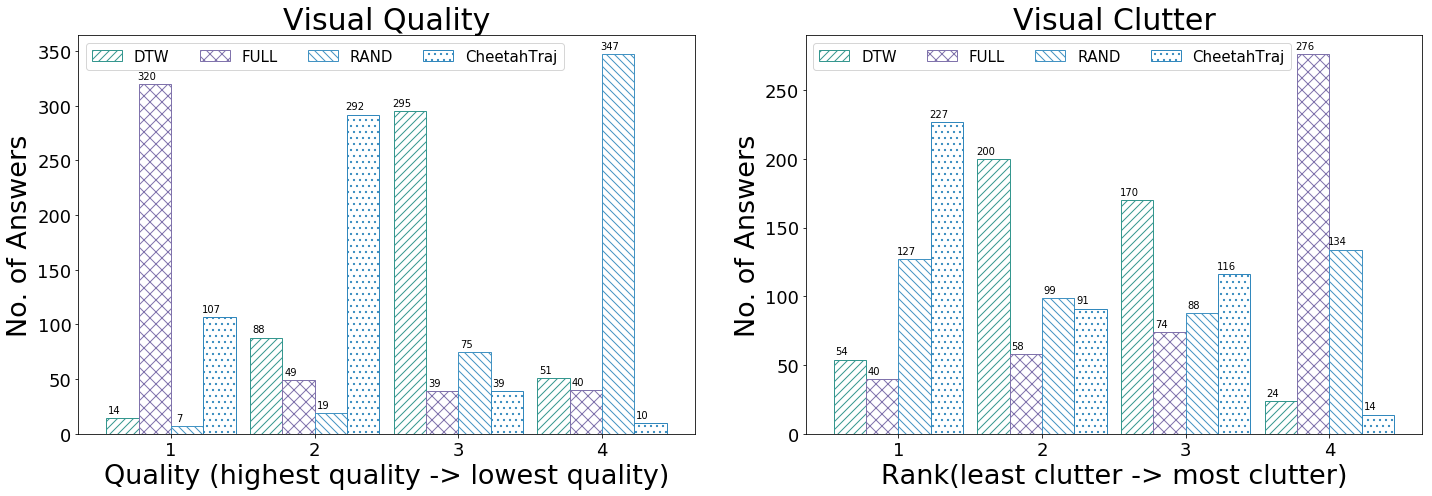
\includegraphics[width=0.6\textwidth]{pictures/user_study/rank.png}
	%\vspace{-3mm}
	\caption{User study, rank distribution.}
	\label{fig:rank}
	%\vspace{-2mm}
\end{figure*}

The left plot of Figure~\ref{fig:rank} reports the quality ranking of 4 methods in T1. The results show that $\full$ ranks the 1st in most cases while $\avats$ usually ranks 1st or 2nd. In contrast, $\mathsf{DTW}$ and $\rand$ rank 3rd and 4th in most cases. This suggests that $\avats$ outperforms $\mathsf{DTW}$ and $\rand$ in visual quality. We also found that $\avats$ ranks 1st mainly for large-scale regions in which there are many trajectories.         

 
%Figure~\ref{fig:rank} left shows the ranking among different methods with x-axis indicating the ranking from the highest quality to the lowest quality and y-axis indicating the selecting number for the specific method and ranking. The visualization of $\full$ has the highest visual quality since it has no information loss according the quality definition. The selection of $\avats$ is mostly concentrated at the first and second, which is closely behind the $\full$. The selections of $\baseline$ and $\rand$ are contracted at the third and fourth respectively, which is confirmed both of these two methods performs worse than $\full$ and $\qtavats$ in guarantee the visual quality.

The right plot of Figure~\ref{fig:rank} reports the anti-visual clutter ranking in T2. The results show that $\full$ has the most severe visual clutter, ranking 4th in most cases. $\rand$ and $\mathsf{DTW}$ reduce visual clutter via sampling, and thus usually rank 2nd and 3rd. $\avats$ is the most successful in reducing visual clutter, ranking 1st in 155 out of the xxx cases.       

%Figure~\ref{fig:rank} right reports the ranking among different methods with x-axis indicating the ranking from the least clutter to the most clutter and y-axis indicating the total selecting number for the specific method and ranking. We observe that the $\qtavats$ is ranked at the first 155 times which is significantly more than the other methods. The number it ranks at the second, third and last are 68, 96 and 14. There is no doubt that the visualization of $full$ suffers the most sever visual clutter problem because 210 of 333 total answers rank $full$ at the fourth, while other methods can be used to help to reduce the visual clutter.

We report the frequency each method is selected as acceptable and why a method is not selected for T3 using bar chart in Figure~\ref{fig:accept_rate}. Each column corresponds to a method and from left to right, the lengths of the bars means ``favorable'', ``not favorable due to visual clutter'', ``not favorable due to poor visual quality'' and ``not favorable for other reasons''. The results show that $\avats$ is acceptable in 85\% of the cases, and the other methods have significantly lower acceptance rate than $\avats$.      




\begin{figure}[t]
	\centering
	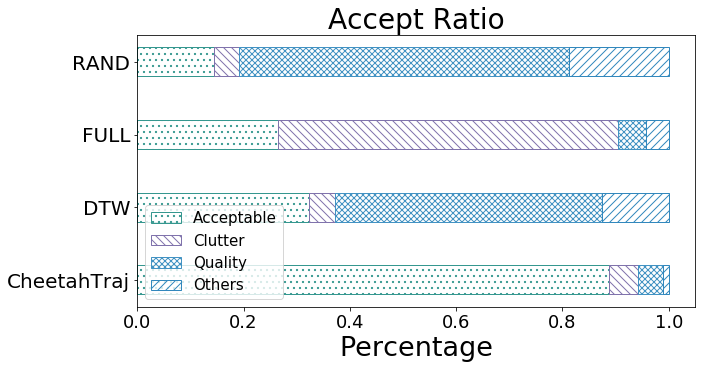
\includegraphics[width=0.35\textwidth]{pictures/user_study/accept_rate.png}
	%\vspace{-5mm}
	\caption{User study, accept rate.}
	\label{fig:accept_rate}
	%\vspace{-8mm}
\end{figure}






\subsection{Quantitative Evaluation}\label{sec:quality}
In this part, we quantitatively evaluate our proposals on the \pt{}, \cd{} and \sz{} trajectory datasets from two aspects:
(i) visual quality and (ii) running time.

\begin{figure}[t]
	\centering
	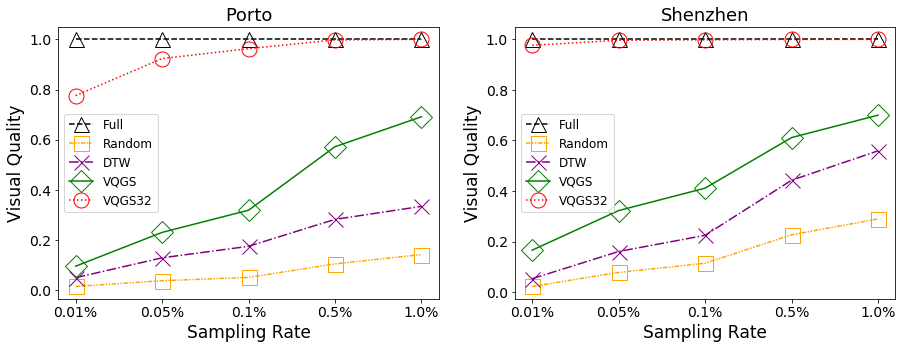
\includegraphics[width=0.5\textwidth]{pictures/quantitative_study_icde/rate_quality.png}
	\vspace{-8mm}
	\caption{Visual quality vs. sampling rates(T1).}
	\label{fig:sample_quality}
	\vspace{-3mm}
\end{figure}

\begin{figure}[t]
	\centering
	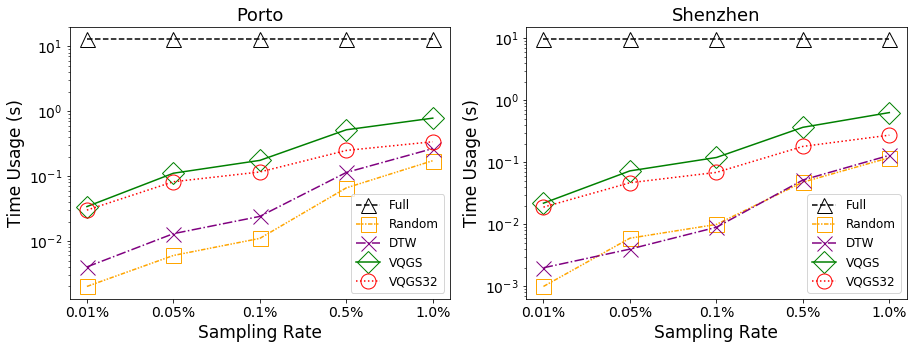
\includegraphics[width=0.5\textwidth]{pictures/quantitative_study_icde/rate_rendertime.png}
	\vspace{-8mm}
	\caption{Rendering time vs. sampling rates(T1).}
	\label{fig:rate_quality}
	\vspace{-3mm}
\end{figure}


\begin{figure}[t]
	\centering
	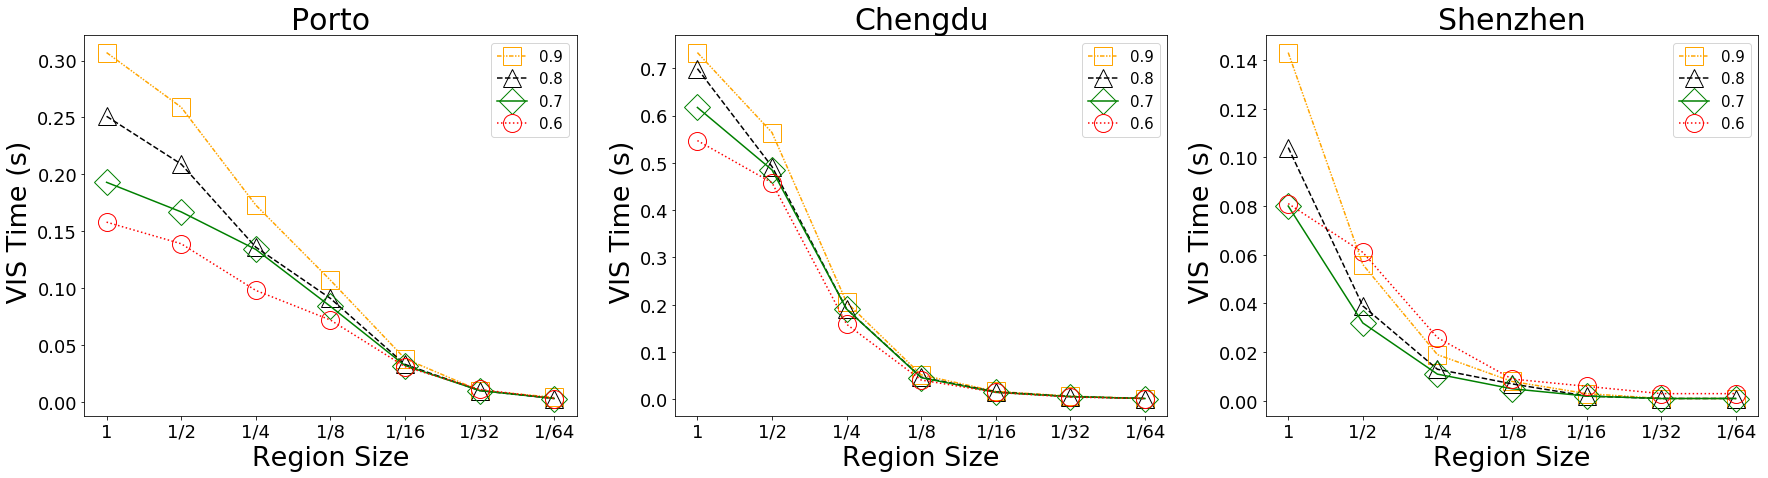
\includegraphics[width=0.5\textwidth]{pictures/quantitative_study_icde/size_rendertime.png}
	\vspace{-8mm}
	\caption{Region size vs. response time(T2).}
	\label{fig:size_rendertime}
	\vspace{-3mm}
\end{figure}

\begin{figure}[t]
	\centering
	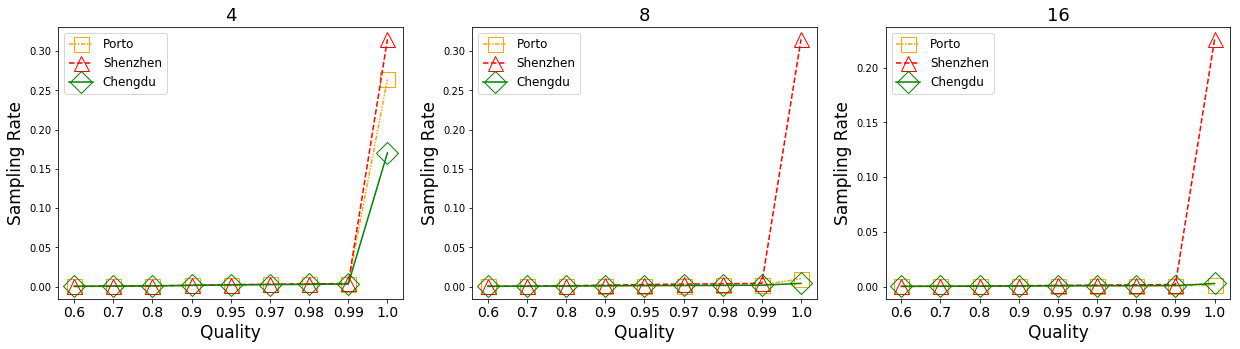
\includegraphics[width=0.5\textwidth]{pictures/quantitative_study_icde/quality_rate.png}
	\vspace{-8mm}
	\caption{Region size vs. response time(T3).}
	\label{fig:quality_rate}
	\vspace{-3mm}
\end{figure}

\begin{figure}[t]
	\centering
	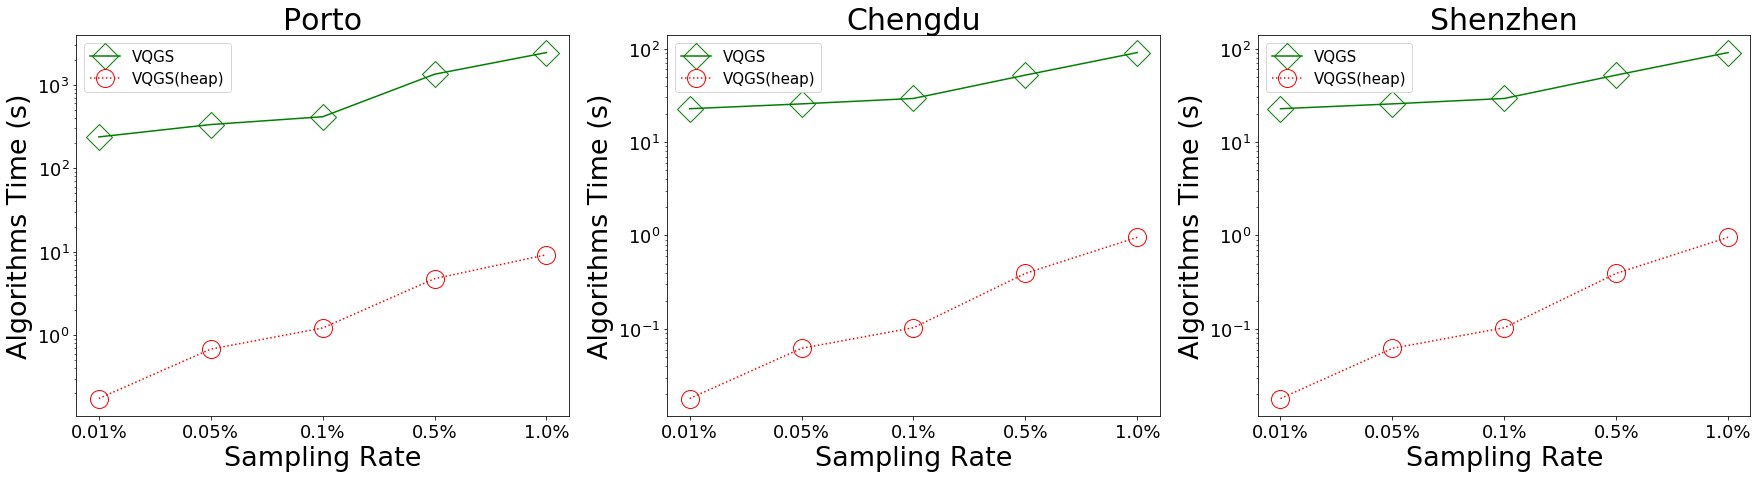
\includegraphics[width=0.5\textwidth]{pictures/quantitative_study_icde/rate_algtime.png}
	\vspace{-8mm}
	\caption{Sampling rate vs. algorithms time(T4).}
	\label{fig:rate_algtime}
	\vspace{-3mm}
\end{figure}
%\begin{figure}[t]
%	\centering
%	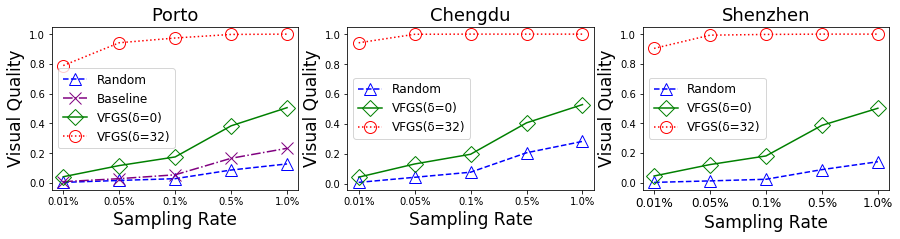
\includegraphics[width=0.5\textwidth]{pictures/quantitative_study_icde/sample_quality.png}
%	\vspace{-8mm}
%	\caption{Visual quality vs. sampling rates.}
%	\label{fig:sample_quality}
%	\vspace{-3mm}
%\end{figure}

%\begin{figure}[t]
%	\centering
%	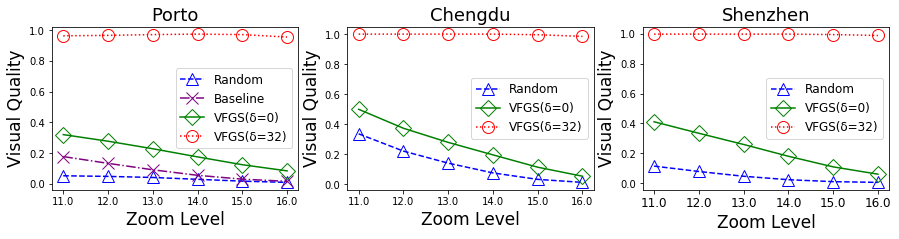
\includegraphics[width=0.5\textwidth]{pictures/quantitative_study_icde/zoom_quality.png}
%	\vspace{-8mm}
%	\caption{Visual quality vs. zoom level.}
%	\label{fig:zoom_quality}
%	\vspace{-3mm}
%\end{figure}

\stitle{Visual quality evaluation}
We evaluate the quality of proposed methods from two aspects: (i) the quality vs different zoom levels; (ii) the quality vs different sampling rates.
Visual quality is defined as the $1-loss$, in which $loss$ is the quality loss function in Equation~\eqref{eqref:loss}. The visualization using the full dataset is used as the ground-truth. 


We report the \textit{visual quality} of different visualization methods in Figure~\ref{fig:sample_quality} with a given sampling $\alpha=0.1\%$. 
The results show that $\rand$ always has the lowest visual quality. $\baseline$ is better than $\rand$ which is also confirmed by case study. Furthermore $\vats$ has better visual quality than $\baseline$ but is significantly outperformed by $\avats$. We also observed that all of the methods across the three dataset have the similar trends: the performance increases when the sampling rate increases.

Figure~\ref{fig:zoom_quality} demonstrates the relationship between visual quality and zoom level. In general, with the increase of the zoom level(zoom into the details), the visual quality drops.
We set the sampling rate $\alpha=1\%$. The results show that $\rand$ always has the lowest  visual quality. $\baseline$ performs better than $\vats$ and $\vats$ is better than $\baseline$. Moreover, $\avats$ has a much higher score than $\vats$. With $\delta=32$ , the minimum visual quality values of $\avats$ are 0.955, 0.985, and 0.989 for \pt{}, \cd{} and \sz{}, respectively. Moreover, the quality of all methods increases when the zoom level drops, which in line with Theorem~\ref{the:level}.



\stitle{Running time evaluation}

%\begin{figure}[t]
%	\centering
%	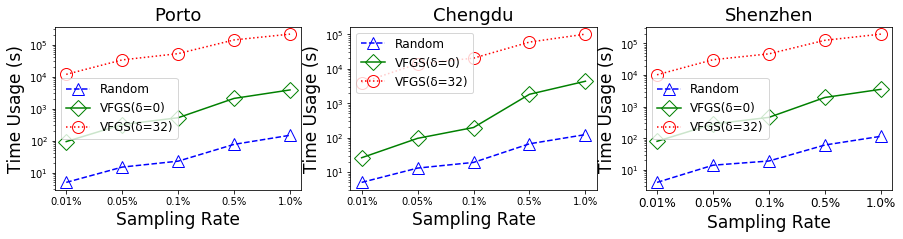
\includegraphics[width=0.5\textwidth]{pictures/quantitative_study_icde/sample_time.png}
%	\vspace{-8mm}
%	\caption{Time usage vs. sampling rates.}
%	\label{fig:sample_time}
%	\vspace{-3mm}
%\end{figure}

%\begin{figure}
%	\centering
%	\small
%	\begin{tabular}{cc}
%		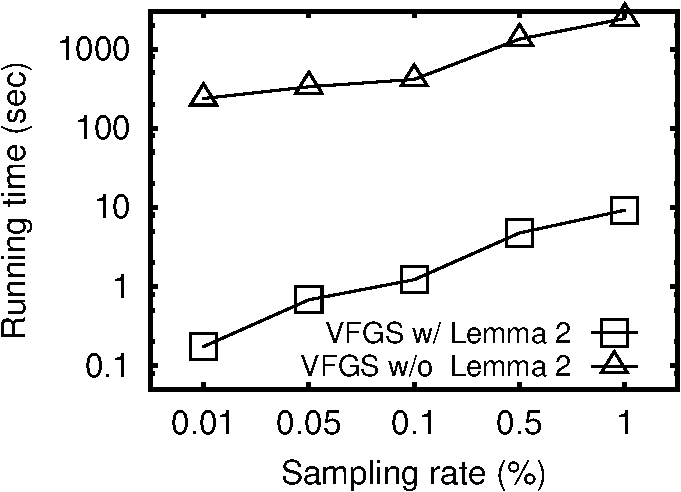
\includegraphics[width=0.44\columnwidth]{pictures/tporto}
%		&
%		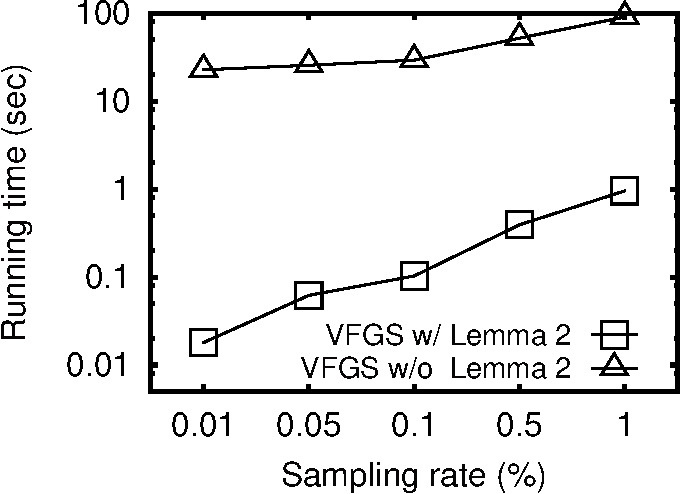
\includegraphics[width=0.44\columnwidth]{pictures/tshenzhen}
%		\\
%		(A) \pt{}
%		&
%		(B) \sz{}	
%	\end{tabular}
%	\vspace{-3mm}
%	\caption{Running time of $\vats$ w/ and w/o Lemma~\ref{lem:submodular}.}
%	\label{fig:cost}
%	\vspace{-6mm}
%\end{figure}
\QM{unfininshed}
We first conduct an experiment to evaluate the rendering cost by datasize. We vary the number of trajectories from 1000 to 1 million, which are randomly selected from \pt{} dataset. The experimental results are summarized in Table~\ref{tab:gpu}. We observe that the rendering cost is linear with the input data trajectories.

We first report the running time of our $\vats$ algorithm in Figure~\ref{fig:cost} by varying the sampling rate from $0.01\%$ to $1\%$. The results show that $\vats$ is quite slow without the submodularity of contribution value, which agrees with Lemma~\ref{lem:submodular} in Section~\ref{sec:opt}.
Then we shown the total time usage with sampling rate as Figure~\ref{fig:sample_time}. {*******}

The optimized $\vats$ (e.g., $\vats$ with Lemma~\ref{lem:submodular}) outperforms $\vats$ by one to three orders of magnitudes on both datasets. The result show that running time of our $\vats$ algorithm is below 1 second in most cases. We have shown that $\vats$ provides good visualization performance with a low sampling rate (e.g., $0.1\%$ or $1\%$) in Section 6.1 and 6.2,  and Table~\ref{tab:gpu} suggests that the rendering latency scales almost linearly with dataset cardinality. By significantly reducing the dataset cardinality with sampling, $\vats$ can effectively reduces the rendering latency to make interactive visualization possible without sacrificing visual quality. For example, rendering the full $\pt{}$ dataset takes about \QM{34 seconds}, with a sampling rate of $1\%$, $\vats$ can bring down the rendering latency to less than 1 second.

\begin{table}
	\centering
	\small
	\caption{Visualization rendering cost}
	\begin{tabular}{|c|c|c|c|c|} \hline
		No. Trajs & GPS points & Mapping (s) & Rendering (s) & Total (s)\\ \hline
		1,000& 31,300 & 0.027 & 0.003 & 0.03 \\ \hline
		10,000& 31,6531 & 0.169 & 0.005 & 0.174\\ \hline
		100,000& 316,7120 & 1.701 & 0.057 & 1.758 \\ \hline
		1,000,000& 31,646,379 & 15.562 & 0.592 & 16.154 \\ \hline
	\end{tabular}	\label{tab:gpu}
\end{table}

